\subsection{Odabir plana ishrane}

Klijent nakon uspešnog registrovanja i prijavljivanja u sistem treba da odabere plan ishrane. Da bi sam proces bio lakši i pregledniji korisniku za korišćenje podeljen je na više smislenih ekrana tj. etapa.
\begin{itemize}
    \item Tip ishrane, broj ljudi i broj recepata za nedelju (slika \ref{fig:SelectMealPlanScreen1})
    \item Detalji o dostavi (slika \ref{fig:SelectMealPlanScreen2})
    \item Detalji o kreditnoj kartici (slika \ref{fig:SelectMealPlanScreen3})
    \item Recepti za narednu nedelju (slika \ref{fig:SelectMealPlanScreen4})
\end{itemize}
Nakon potvrde izmene klijent dobija potvrdu da su podaci uspešno sačuvani. (slika \ref{fig:SelectMealPlanScreen5})

\begin{figure}[H]
	\begin{center}
		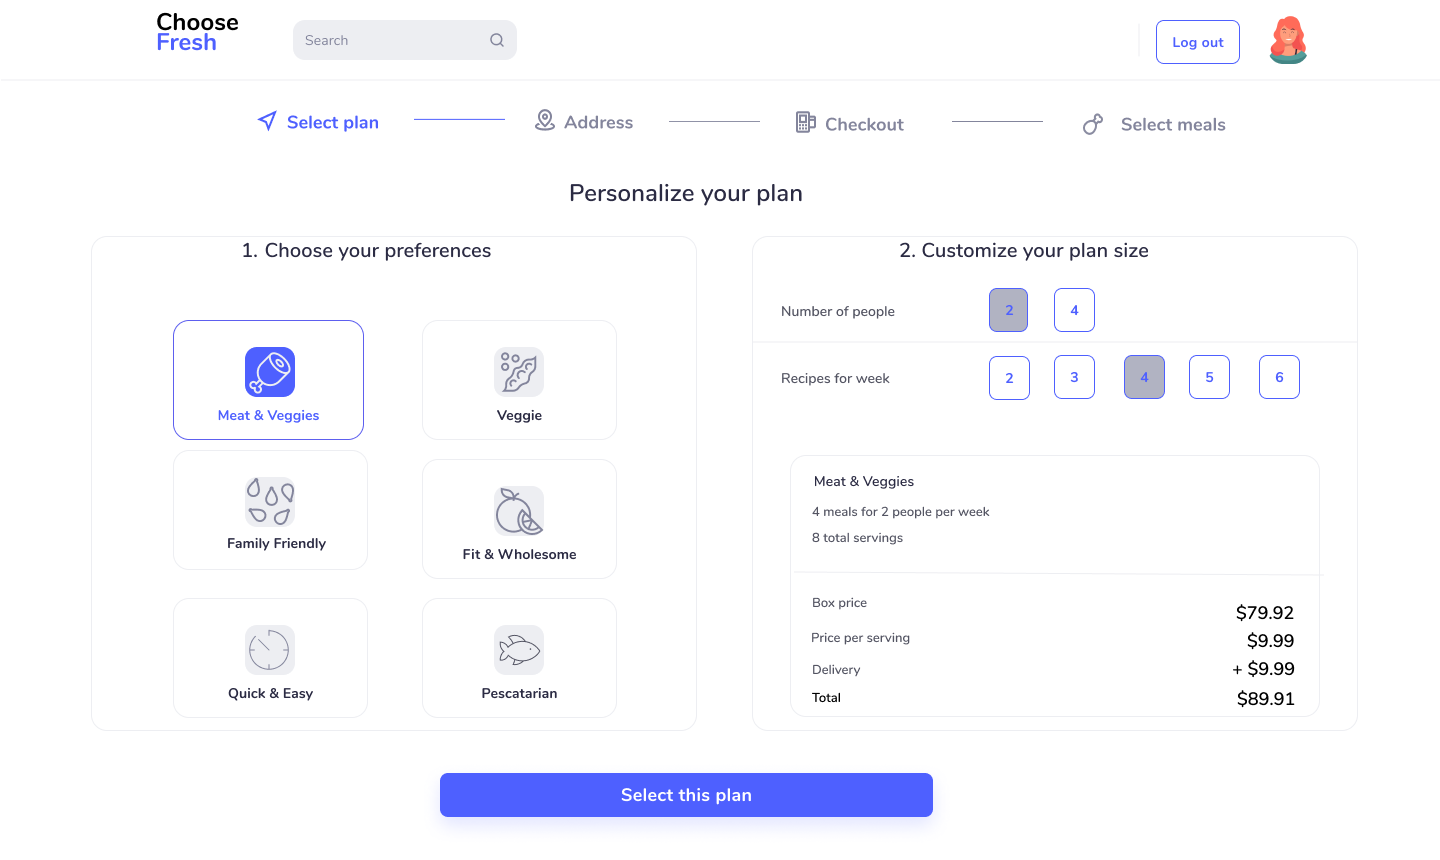
\includegraphics[width=\textwidth]{UI/Select Meal Plan (Screen 1).png}
    		\caption{Odabir tipa plana ishrane, broja ljudi i broja recepata}
    \label{fig:SelectMealPlanScreen1}
    \end{center}
\end{figure}

\begin{figure}[H]
	\begin{center}
		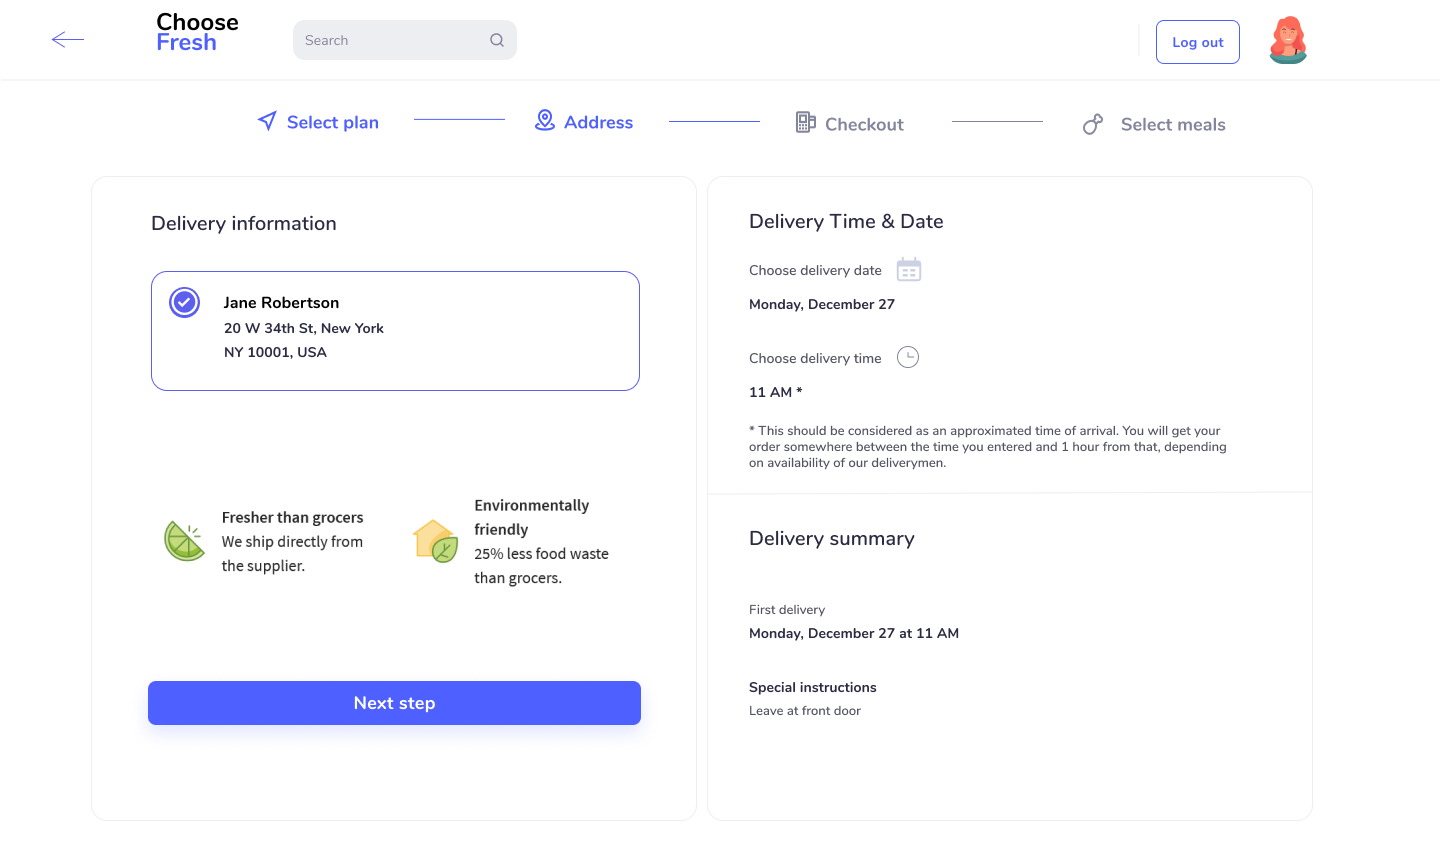
\includegraphics[width=\textwidth]{UI/Select Meal Plan (Screen 2).png}
    		\caption{Unos detalja o dostavi}
    \label{fig:SelectMealPlanScreen2}
    \end{center}
\end{figure}

\begin{figure}[H]
	\begin{center}
		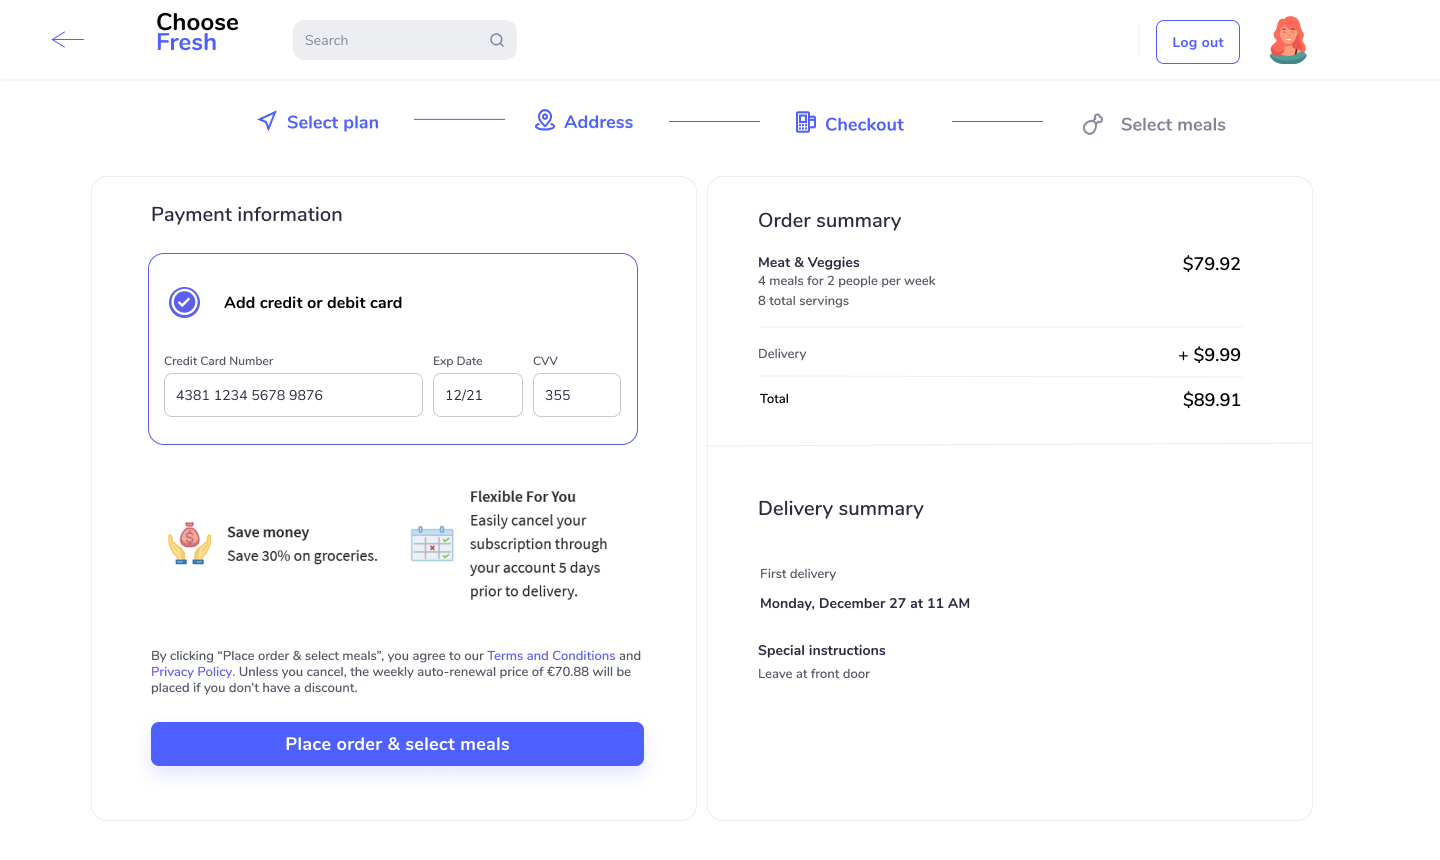
\includegraphics[width=\textwidth]{UI/Select Meal Plan (Screen 3).png}
    		\caption{Unos detalja o kreditnoj kartici}
    \label{fig:SelectMealPlanScreen3}
    \end{center}
\end{figure}

\begin{figure}[H]
	\begin{center}
		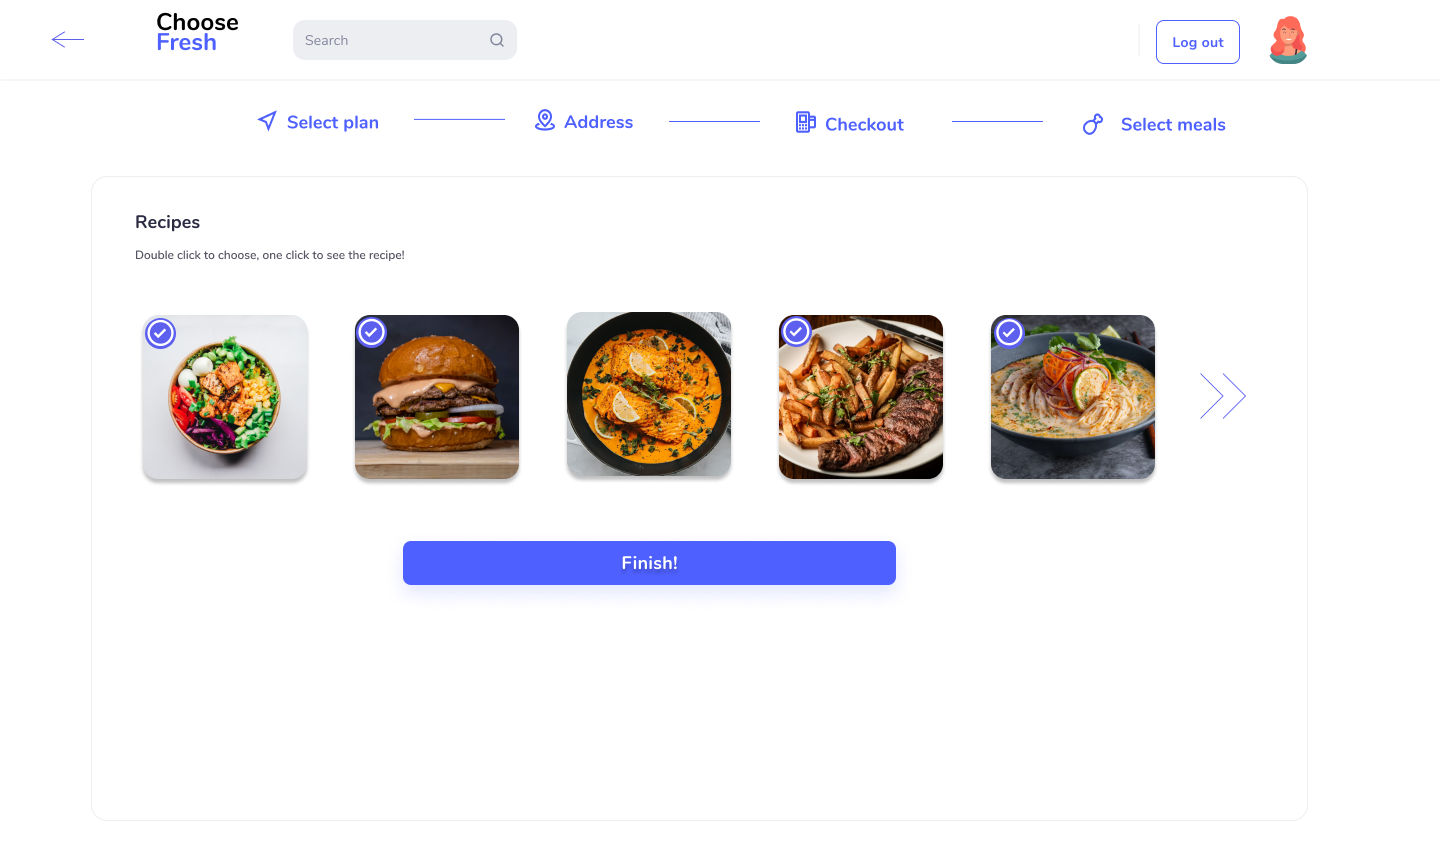
\includegraphics[width=\textwidth]{UI/Select Meal Plan (Screen 4).png}
    		\caption{Izbor recepata}
    \label{fig:SelectMealPlanScreen4}
    \end{center}
\end{figure}

\begin{figure}[H]
	\begin{center}
		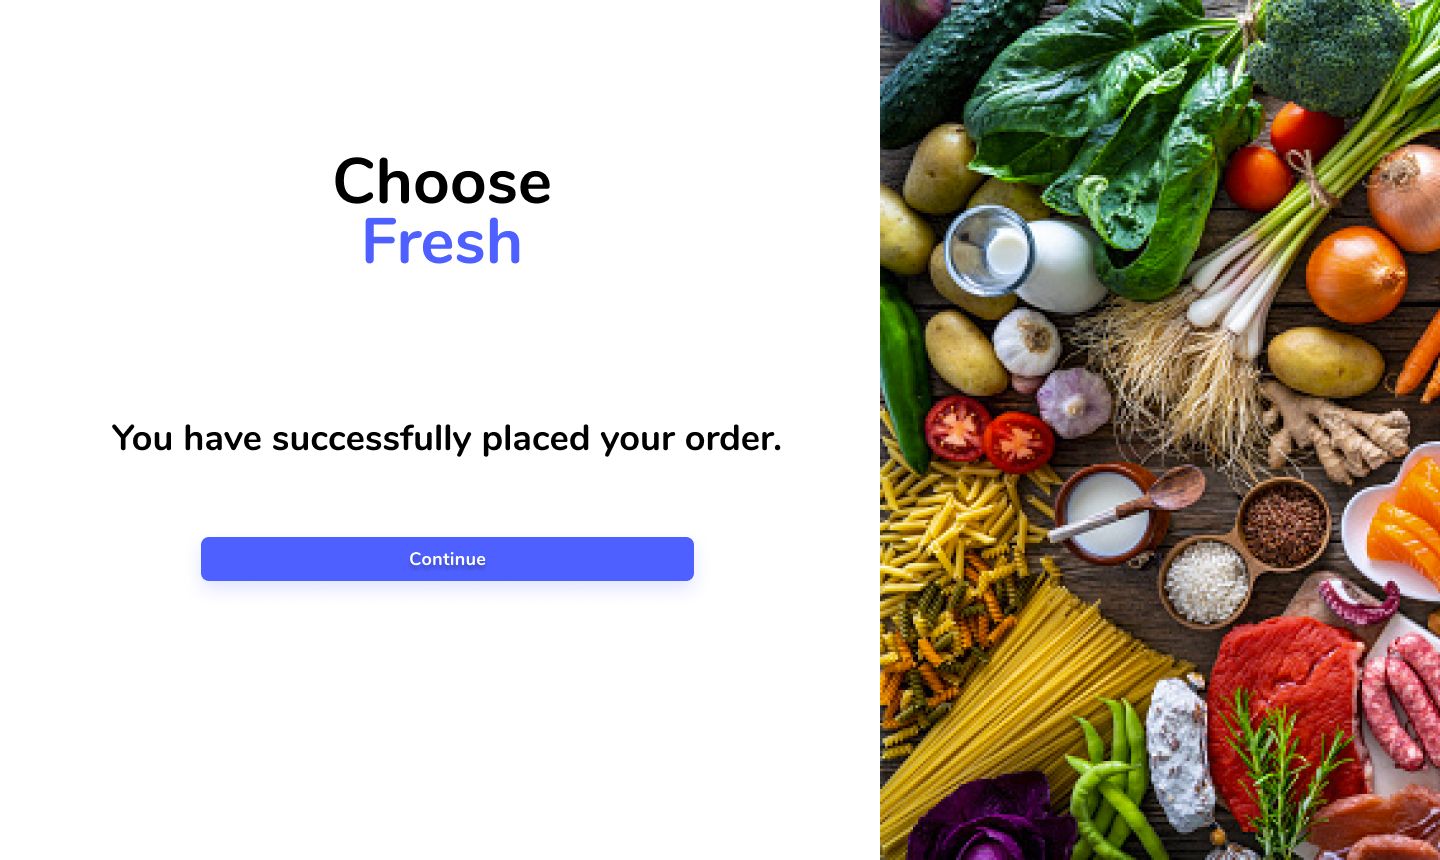
\includegraphics[width=\textwidth]{UI/Select Meal Plan (Screen 5).png}
    		\caption{Potvrda o uspešnom odabiru plana ishrane}
    \label{fig:SelectMealPlanScreen5}
    \end{center}
\end{figure}
